\documentclass[dvipdfmx, fleqn]{jsarticle}
%% packages and libraries
\usepackage{amsmath, amssymb, amsfonts, mathtools, cases, mathrsfs}	%math
\usepackage{physics}
\usepackage{fancyhdr, lastpage}										%header and footer
%\usepackage{titlesec}													%title design
\usepackage{hyperref}													%link
\usepackage{url}														%URL
\usepackage{pxjahyper}												%arrow Japanese for hyperref
\usepackage[table]{xcolor}											%tables and color
\usepackage{longtable, float, multirow, array, listliketab, enumitem, tabularx}	%tables
\usepackage{flafter}
\usepackage{comment}												%comment out over 2 lines
\usepackage{graphicx}													%figure
\usepackage{subcaption, wrapfig}									%configuration
\usepackage{tikz}														%TikZ
\usetikzlibrary{calc, patterns, decorations, decorations.pathmorphing, angles, backgrounds, shadows, positioning, shapes.geometric, arrows}
\usepackage{algorithm, algorithmic}
\usepackage{pdfpages}												%include PDF
\usepackage{import, grffile}											%management files
\usepackage{standalone}
\usepackage[T1]{fontenc}											%fonts
\usepackage{textcomp}
\usepackage[utf8]{inputenc}
\usepackage{lmodern}
\usepackage{mathptmx}
\usepackage[scaled]{helvet}
\renewcommand{\ttdefault}{pcr}
\usepackage[deluxe]{otf}
\usepackage[noalphabet]{pxchfon}
\usepackage{bm}
\usepackage{lscape}
\usepackage{siunitx}													%units
\usepackage{bigstrut}


%% set up for hyperref
\hypersetup{
	bookmarksnumbered = true,
	hidelinks,
	colorlinks = true,
	linkcolor = black,
	urlcolor = cyan,
	citecolor = black,
	filecolor = magenta,
	setpagesize = false,
	pdftitle = {},
	pdfauthor = {Morita},
	pdfkeywords = {},
	}


%% set up for siunitx
\sisetup{%
	%detect-family = true,						%bold
	detect-inline-family = math,
	detect-weight = true,
	detect-inline-weight = math,
	%input-product = *,							%multiply by *
	quotient-mode = fraction,						%fraction by /
	fraction-function = \frac,
	inter-unit-product = \ensuremath{\hspace{-1.5pt}\cdot\hspace{-1.5pt}},	%devide different units by \cdot
	per-mode = symbol,%							%devide different unit by /
	product-units = single,%						%
	}


%% fonts
\setminchofont{ipam.ttf}
\setgothicfont{ipag.ttf}
\fontsize{14Q}{30H}


%% layout
%space between letters
\kanjiskip 0zw plus 1zw minus 0zw
\xkanjiskip 0.25zw plus 1pt minus 1pt
%line skip
\setlength{\lineskiplimit}{2pt}
\setlength{\lineskip}{2pt}
%indent
\setlength{\parindent}{1zw}
\setlength{\mathindent}{5zw}


%put citation mark on index zone
\bibliographystyle{junsrt}


%hyphen for math mode
\DeclareMathSymbol{\mhyphen}{\mathalpha}{operators}{`-}


%circle text
\newcommand{\ctext}[1]{\raise0.2ex\hbox{\textcircled{\scriptsize{#1}}}}


%unit of formulas 〔roman〕
\newcommand{\unitis}[1]{%
	\text{〔\si{#1}〕}
	}


\title{Auto-Encoding Variational Bayes 日本語訳}
\date{2019-07-10}
\author{
    森田涼介
    }
\begin{document}

\maketitle

\vspace{\baselineskip}
\begin{center}
\Large
    Auto-Encoding Variational Bayes

\large
\vspace{\baselineskip}
    Diederik P. Kingma
    \qquad
    Max Welling
 
\vspace{\baselineskip}
    2014-03-01
\end{center}
\vspace{2\baselineskip}


\begin{abstract}
    有向確率モデルにおいて,
    潜在変数が連続でその事後分布が計算不可能であり,
    かつデータセットが大規模なとき,
    その学習及び推論はどのように行ったらよいだろうか。
    我々は,この学習と推論について,
    データセットが大きくなっても適用可能で,
    また計算不可能な場合でも微分可能性についてある緩い条件が成立すれば機能する,
    確率的変分アルゴリズムを導入する。
    我々は次の2つのことを達成した。
    1つは,変分下限を再パラメータ化することで,
    下限の推定を可能にしたことである。
    なお,これは通常の確率的勾配法を用いて直接的に最適化することができる,
    もう1つは,各データについて連続潜在変数を持つi.i.d.なデータセットについて,
    効率的な事後推定を可能にしたことである。
    これは,下限の推定器を用い,近似的推論モデル(認識モデルとも呼ばれる)を計算不可能な事後分布に適用することで達成される。
    この理論の利点は実験の結果に表れている。
\end{abstract}



\section{序論}

有向確率モデルにおいて,
その連続潜在変数またはパラメータが計算不可能な事後分布を持つとき,
近似的推論と学習はどのように行ったらよいだろうか。
変分ベイズ(variational Bayesian, VB)的アプローチでは,
計算不可能な事後分布に対する近似の最適化が行われる。
通常の平均場的なアプローチでは,
事後分布の近似についての期待値の解析解が必要となるが,
一般にはこれもイントラクタブルである。
我々は,変分下限の再パラメータ化によって,
いかにして単純で微分可能な下限の不偏推定器を得られるのかを示す。
このSGVB (Stochastic Gradient Variational Bayes)推定器は,
連続潜在変数またはパラメータを持つほとんどのモデルにおいて効率の良い近似的事後推定に用いることができ,
また,通常の確率的勾配上昇法を用いて最適化できる。

各データに対し連続な潜在変数があり,かつi.i.d.なデータセットの場合について,
我々は自己符号化変分ベイズ(AutoEncoding Variational Bayes, AEVB)アルゴリズムを提案する。
AEVBアルゴリズムによって,学習・推論を非常に効率よく行うことができるようになる。
これは,SGVB推定器を用いて認識モデルを最適化することによって達成される。
この認識モデルでは,
各データに対して計算コストの高い反復的推論法(MCMCなど)を用いず,
モデルのパラメータを効率よく学習できるような,
単純な伝承サンプリングを用いることによって,
非常に効率的な近似的事後推定を行うことができる。
学習された近似的事後推定モデルは,
認識・ノイズ除去・表現学習・可視化などの,
様々なタスクに用いることができる。
認識モデルにニューラルネットワークを用いたとき,
これを変分自己符号化器(variational auto-encoder)と呼ぶ。



\section{手法}

この節では,
連続型潜在変数を持つ様々な有向グラフィカルモデルに対して,
下限推定器(確率的目的関数)を得られうような手法を導入する。
いま,各データについて潜在変数があるi.i.d.なデータセットという一般の場合を考える。
最尤推定や最大事後確率推定を(大域的な)パラメータに対して行い,
また変分推論を潜在変数に対して行う。
これは例えば,変分推論を大域的なパラメータに適用する場合にも自然に拡張できる。
このアルゴリズムは付録に示したが,実験は今後の展望とした。
以下では簡単のため定常なデータセットを仮定するが,
この手法はストリーミングデータのようなオンラインの非定常なデータセットにも適用できる。


\subsection{問題の概要}

\(N\)個のi.i.d.な変数\(\bm{x}\)から成るデータセット\(\bm{X} = \qty{\bm{x}^{(i)}}_{i=1}^{N}\)を考える。
なお,\(\bm{x}\)は連続的でも離散的でもよい。
いま,そのデータは,
観測されない連続型確率変数\(\bm{z}\)を含む,
ある確率過程から生成されていると仮定する。
その確率過程には次の2段階がある。
\begin{enumerate}[label=(\arabic*)]
    \item \(\bm{z}^{(i)}\)がある事前分布\(p_{\theta^*} (\bm{z})\)から生成される
    \item \(\bm{x}^{(i)}\)がある条件付確率\(p_{\theta^*} (\bm{x}|\bm{z})\)から生成される
\end{enumerate}
ここで,
事前分布\(p_{\theta^*} (\bm{z})\)と尤度\(p_{\theta^*} (\bm{x}|\bm{z})\)は
分布\(p_{\theta} (\bm{z})\)と\(p_{\theta} (\bm{x}|\bm{z})\)のparametric familyから得られ,
また,それらの確率密度関数は\(\theta\)と\(\bm{z}\)の両方について
ほとんど至るところで微分可能であると仮定する。
不運なことに,この過程の多くの部分が,我々から見えないところで起こるものである。
つまり,
真のパラメータ\(\theta^*\),及び潜在変数\(\bm{z}^{(i)}\)について,我々は知りえない。

非常に重要なことだが,我々は,一般的に行われるような周辺確率や事後確率に関する単純化を仮定しない。
むしろここでは,以下のような場合でも機能するような,
一般的なアルゴリズムが求められているのである。

\begin{enumerate}
    \item 計算不可能性 \\
        周辺尤度の積分\(p_{\theta} (\bm{x}) = \int p_{\theta} (\bm{z}) p_{\theta} (\bm{x}|\bm{z}) \dd\bm{z}\)がイントラクタブルな場合(このとき周辺尤度の値を求めたり微分したりすることはできない)。
        このとき,真の事後確率密度\(p_\theta (\bm{z}|\bm{x}) = p_{\theta} (\bm{x}|\bm{z}) p_{\theta} (\bm{z}) / p_{\theta} (\bm{x})\)は計算不可能である(このときEMアルゴリズムは使用できない)。
        また,どんな平均場変分ベイズアルゴリズムに対しても,その積分は計算不可能となる。
        こういった計算不可能性は一般に起こりうるもので,
        尤度関数\(p_{\theta} (\bm{x}|\bm{z})\)にある程度複雑なもの,
        例えば非線形な隠れ層を持つニューラルネットワークを
        用いた場合などに現れる性質である。
    \item 大規模データセット \\
        データが非常に多く,
        バッチ最適化の計算コストが高くなりすぎる場合。
        このとき,ミニバッチまたはデータ1つを用いてパラメータを更新したい。
        モンテカルロEM法などのサンプリングによる方法は,
        各データに対し計算コストの高いサンプリングを反復的に行うため,
        一般にかなり遅くなってしまう。
\end{enumerate}

我々は上記のような状況に関する以下の3つの問題について関心があり,
その解決法を提案する。

\begin{enumerate}
    \item
        パラメータ\(\theta\)に対して,どう効率よくMLEやMAP推定の近似を行うか。
        パラメータ自身も,自然の作用などを分析するときなどは関心の対象となりうる。
        また,パラメータによって,
        非明示的な確率過程を模倣することが可能になり,
        実データに似た人工データを作り出すことができるようになる。
    \item
        観測値\(\bm{x}\)が与えられたとき,ある\(\theta\)に対して,
        潜在変数\(\bm{z}\)の事後分布の近似をどう効率よく行うか。
        これは,符号化や表現学習をするときに有用である。
    \item
        変数\(\bm{x}\)の周辺確率の近似をどう効率よく行うか。
        これを行うことにより,
        \(\bm{x}\)に関する事前分布が必要となるような問題に対応できるようになる。
        例えば,コンピュータービジョンにおける応用例として,
        画像のノイズ除去や修復,超解像といったものが挙げられる。
\end{enumerate}

上記のような問題を解くために,
認識モデル\(q_{\phi} (\bm{z} | \bm{x})\)を導入しよう。
これは,計算不可能な真の事後分布\(p_{\theta} (\bm{z} | \bm{x})\)の近似である。
平均場変分推論における事後分布の近似とは対照的に,
このモデルは因子分解可能である必要はなく,
またそのパラメータ\(\phi\)は閉形式の期待値から計算されるものでもない。
その代わりとして,
認識モデルのパラメータ\(\phi\)を生成モデルのパラメータ\(\theta\)とまとめて学習する方法を提案する。

符号理論的な観点からすると,
観測されない変数\(\bm{z}\)は潜在表現,
または「符号」として解釈することができる。
そこで本論文では,
認識モデル\(q_{\phi} (\bm{z} | \bm{x})\)を,確率的「符号器」とも呼ぶことにする。
これは,このモデルが,あるデータ\(\bm{x}\)が与えられたとき,
その\(\bm{x}\)を生成する元となった符号\(\bm{z}\)の取りうる値の分布(例えばガウス分布など)を与えるからである。
同様に,\(p_{\theta} (\bm{x} | \bm{z})\)を確率的「復号器」と呼ぶこととする。
これは,このモデルが,ある符号\(\bm{z}\)を与えられたとき,
対応する\(\bm{x}\)の値の取りうる範囲の分布を与えるからである。

\begin{figure}
    \centering
    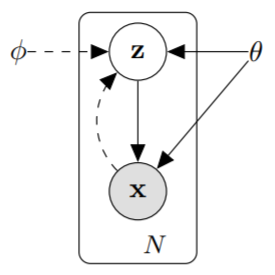
\includegraphics[clip, width=5cm]{../figures/graphical_model}
    \caption{
        対象としている有向グラフモデル。
        実線は生成モデル\(p_{\theta} (\bm{z}) p_{\theta} (\bm{x} | \bm{z})\)を表し,
        破線は計算不可能な事後分布\(p_{\theta} (\bm{z} | \bm{x})\)の変分近似\(q_{\phi} (\bm{z} | \bm{x})\)を表す。
        変分パラメータ\(\phi\)は生成モデルのパラメータ\(\theta\)とまとめて学習される。
        }
    \label{fig:graphical_model}
\end{figure}



\subsection{変分下限}

周辺尤度は,各データの周辺尤度の積で表される。
つまり,
\begin{equation*}
    \log{p_{\theta} (\bm{x}^{(1)},\ \cdots,\ \bm{x}^{(N)})} = \sum_{i=1}^{N} \log{p_{\theta} (\bm{x}^{(i)})}
\end{equation*}
である。
また,次が成立する。
\begin{equation}
    \log{p_{\theta} (\bm{x}^{(i)})}
        = D_\mathrm{KL} (q_{\phi} (\bm{z} | \bm{x}) || p_{\theta} (\bm{z} | \bm{x}^{(i)}))
            + \mathcal{L} (\theta, \phi; \bm{x}^{(i)})
    \label{eq:marginal_log_likelihood}
\end{equation}
右辺第一項は,真の事後分布から測った近似的事後分布のKL情報量である。
このKL情報量は非負であることから,
右辺第二項の\(\mathcal{L} (\theta, \phi; \bm{x}^{(i)})\)は,
データ\(i\)の周辺尤度に関する(変分)下限と呼ばれる。
これは次のように表される。
\begin{equation}
    \log{p_{\theta} (\bm{x}^{(i)})}
        \ge \mathcal{L} (\theta, \phi; \bm{x}^{(i)})
        = \mathbb{E}_{q_{\phi} (\bm{z} | \bm{x})} \qty[-\log{q_{\phi} (\bm{z} | \bm{x})} + \log{p_{\theta} (\bm{x},\ \bm{z})}]
    \label{eq:derivation_variational_lower_bound}
\end{equation}
また,
\begin{equation}
    \mathcal{L} (\theta, \phi; \bm{x}^{(i)})
        = -D_\mathrm{KL} (q_{\phi} (\bm{z} | \bm{x}^{(i)}) || p_{\theta} (\bm{z}))
            + \mathbb{E}_{q_{\phi} (\bm{z} | \bm{x}^{(i)})} \qty[\log{p_{\theta} (\bm{x}^{(i)} | \bm{z})}]
    \label{eq:variational_lower_bound}
\end{equation}
下限\(\mathcal{L} (\theta, \phi; \bm{x}^{(i)})\)を,
変分パラメータ\(\phi\)と生成パラメータ\(\theta\)について微分し,
最適化することを考える。
しかし,下限の\(\phi\)に関する勾配の計算に少し問題がある。
こういった問題に対する,
通常の(ナイーブな)モンテカルロ勾配推定は次のようになる。
\begin{equation*}
    \grad_{\phi} \mathbb{E}_{q_{\phi} (\bm{z})} \qty[f(\bm{z})]
        = \mathbb{E}_{q_{\phi} (\bm{z})} \qty[f(\bm{z}) \grad_{q_{\phi} (\bm{z})} \log{q_{\phi} (\bm{z})}]
        \simeq \frac{1}{L} \sum_{l=1}^{L} f(\bm{z}) \grad_{q_{\phi} (\bm{z}^{(l)})} \log{q_{\phi} (\bm{z}^{(l)})}
\end{equation*}
ここで,\(\bm{z}^{(l)} \sim q_{\phi} (\bm{z} | \bm{x}^{(i)})\)である。
このように勾配を推定するとバリアンスが非常に大きくなり(例えば[BJP12]),
我々の目的にとっては実用的でないことがわかる。



\subsection{SGVB推定器とAEVBアルゴリズム}

この節では,
下限とそのパラメータについての微分に対して,
実用的な推定法を導入する。
いま,近似的事後分布を\(q_{\phi} (\bm{z} | \bm{x})\)の形式で仮定しているが,
この推定法は\(q_{\phi} (\bm{z})\)の場合,
つまり\(\bm{x}\)について条件を考えない場合にしか適用できないことに注意されたい。
事後分布の推定に関する完全な変分ベイズ法は付録に示した。

2.4節で説明する,事後分布の近似\(q_{\phi} (\bm{z} | \bm{x})\)に関するある緩い条件の下では,
確率変数\(\tilde{\bm{z}} \sim q_{\phi} (\bm{z} | \bm{x})\)を,
(補助)ノイズ変数\(\bm{\epsilon}\)の微分可能な変換\(g_{\phi} (\bm{\epsilon},\ \bm{x})\)を用いて再パラメータ化でき,
\begin{equation}
    \tilde{\bm{z}} = g_{\phi} (\bm{\epsilon},\ \bm{x})
        \quad \text{with} \quad
        \bm{\epsilon} \sim p(\bm{\epsilon})
    \label{eq:reparameterization}
\end{equation}
適切な分布\(p(\bm{\epsilon})\)と関数\(g_{\phi} (\bm{\epsilon},\ \bm{x})\)を選ぶ方法については,2.4節を参照されたい。
いま,これを用いて\(q_{\phi} (\bm{z} | \bm{x})\)に関するある関数\(f(\bm{z})\)の期待値のモンテカルロ推定を定式化すると次のようになる。
\begin{equation}
    \mathbb{E}_{q_{\phi} (\bm{z} | \bm{x}^{(i)})} \qty[f(\bm{z})]
        = \mathbb{E}_{p(\bm{\epsilon})} \qty[f(g_{\phi} (\bm{\epsilon},\ \bm{x}^{(i)}))]
        \simeq \frac{1}{L} \sum_{l=1}^{L} f(g_{\phi} (\bm{\epsilon}^{(l)},\ \bm{x}^{(i)}))
    \quad \text{where} \quad
    \bm{\epsilon}^{(l)} \sim p(\bm{\epsilon}^{(l)})
    \label{eq:expectation}
\end{equation}
この手法を変分下限(式(\ref{eq:derivation_variational_lower_bound}))に適用すると,
確率的勾配変分ベイズ(SGVB)推定器
\(\tilde{\mathcal{L}}^\mathrm{A} (\theta, \phi; \bm{x}^{(i)}) \simeq \mathcal{L} (\theta, \phi; \bm{x}^{(i)})\)が得られ,
\begin{equation}
    \begin{split}
    & \tilde{\mathcal{L}}^\mathrm{A} (\theta, \phi; \bm{x}^{(i)})
        = \frac{1}{L} \sum_{i=1}^{L} \log{p_{\theta} (\bm{x}^{(i)},\ \bm{z}^{(i, l)})} - \log{q_{\phi} (\bm{z}^{(i, l)} | \bm{x}^{(i)})} \\
    & \text{where} \quad
        \bm{z}^{(i, l)} = g_{\phi} (\bm{\epsilon}^{(i, l)},\ \bm{x}^{(i)})
        \quad \text{and} \quad
        \bm{\epsilon}^{(l)} \sim p(\bm{\epsilon})
    \end{split}
    \label{eq:SGVB_estimator_A}
\end{equation}

式(\ref{eq:variational_lower_bound})のKL情報量\(D_\mathrm{KL} (q_{\phi} (\bm{z} | \bm{x}^{(i)}) || p_{\theta} (\bm{z}))\)は
解析的に積分可能(付録B参照)であることが多い。
再構成期待誤差\(\mathbb{E}_{q_{\phi} (\bm{z} | \bm{x}^{(i)})} \qty[\log{p_{\theta} (\bm{x}^{(i)} | \bm{z})}]\)がサンプリングによる推定しか必要としない場合に限るが。
これより,KL情報量の項は,
近似した事後分布を事前分布\(p(\bm{z})\)に近づけ,
\(\phi\)を正則化していると解釈できる。
このことから,式(\ref{eq:variational_lower_bound})に対応した,
もう一つのSGVB推定器
\(\tilde{\mathcal{L}}^\mathrm{B} (\theta, \phi; \bm{x}^{(i)}) \simeq \mathcal{L} (\theta, \phi; \bm{x}^{(i)})\)が得られる。
これは一般の推定器よりもバリアンスが小さくなる傾向にある。
\begin{equation}
    \begin{split}
    & \tilde{\mathcal{L}}^\mathrm{B} (\theta, \phi; \bm{x}^{(i)})
        = - D_\mathrm{KL} (q_{\phi} (\bm{z} | \bm{x}^{(i)}) || p_{\theta} (\bm{z}))
            + \frac{1}{L} \sum_{i=1}^{L} \log{p_{\theta} (\bm{x}^{(i)} | \bm{z}^{(i, l)})} \\
    & \text{where} \quad
        \bm{z}^{(i, l)} = g_{\phi} (\bm{\epsilon}^{(i, l)},\ \bm{x}^{(i)})
        \quad \text{and} \quad
        \bm{\epsilon}^{(l)} \sim p(\bm{\epsilon})
    \end{split}
    \label{eq:SGVB_estimator_B}
\end{equation}
\(N\)個のデータを持つデータセット\(\bm{X}\)のうち複数のデータを用い,
ミニバッチに基づいてデータセット全体の周辺尤度の下限を推定すると次のようになる。
\begin{equation}
    \mathcal{L} (\theta, \phi; \bm{X})
        \simeq \tilde{\mathcal{L}}^{M} (\theta, \phi; \bm{X}^{M})
        = \frac{N}{M} \sum_{i=1}^{M} \tilde{\mathcal{L}} (\theta, \phi; \bm{x}^{(i)})
    \label{eq:variational_lower_bound_minibatch}
\end{equation}
ここで,ミニバッチ\(\bm{X}^{M} = \qty{x^{(i)}}_{i=1}^{M}\)は
\(N\)個のデータを持つデータセット\(\bm{X}\)全体からランダムに\(M\)個選んで作られたものである。
実験において,各データに対するサンプル数\(L\)は,
ミニバッチサイズが十分大きければ,例えば\(M = 100\)ならば,
1としてよいことがわかった。
以上より,
微分\(\grad_{\theta, \phi} \tilde{\mathcal{L}} (\theta; \bm{X}^{M})\)は計算できるようになった。
この勾配はSGDやAdagrad [DHS10]などの確率的最適化法において用いることができる。
確率的勾配を計算する基本的な方法については,アルゴリズム\ref{algo:AEVB_minibatch}を参照されたい。

自己符号化器との接点は,
式(\ref{eq:SGVB_estimator_B})で与えられる目的関数を見ると明らかになる。
第一項(事前分布から測った事後分布の近似のKL情報量)は正則化項として働き,
第二項は負の再構成期待誤差となる。
関数\(g_{\phi} (.)\)はデータ\(\bm{x}^{(i)}\)とノイズベクトル\(\bm{\epsilon}^{(l)}\)をそのデータの近似的事後分布のある標本に写像するように選ばれる。
ここで,
\(\bm{z}^{(i, l)} = g_{\phi} (\bm{\epsilon}^{(l)},\ \bm{x}^{(i)})
\ \ \text{where}\ \ 
\bm{z}^{(i, l)} \sim q_{\phi} (\bm{z} | \bm{x}^{(i)})
\)
である。
続いて,標本\(\bm{z}^{(i, l)}\)は関数\(\log{p_{\theta} (\bm{x}^{i} | \bm{z}^{(i, l)})}\)に入力される。
ここで,関数\(\log{p_{\theta} (\bm{x}^{(i)} | \bm{z}^{(i, l)})}\)は
\(\bm{z}^{(i, l)}\)を与えられたときの生成モデルにおける,
データ\(\bm{x}^{(i)}\)の確率密度(質量)である。
この項は,自己符号化器における負の「再構成誤差」に対応する。

\begin{algorithm}
    \caption{
        自己符号化変分ベイズ(AEVB)アルゴリズムのミニバッチ版。
        2.3節の2つのSGVB推定器は両方とも用いられている。
        実験では\(M = 100,\ L = 1\)とした。
        }
    \label{algo:AEVB_minibatch}
    \begin{algorithmic}
        \STATE \(\theta,\ \phi \leftarrow \text{Initialize parameters}\)
        \REPEAT
            \STATE \(\bm{X}^{M} \leftarrow \text{Random minibatch of \(M\) datapoints (drawn from full dataset)}\)
            \STATE \(\bm{\epsilon} \leftarrow \text{Random samples from noise distribution } p(\bm{\epsilon})\)
            \STATE \(g \leftarrow \grad_{\theta, \phi} \tilde{\mathcal{L}}^{M} (\theta, \phi; \bm{X}^{M}, \bm{\epsilon}) \text{(Gradients of minibatch estimator (\ref{eq:variational_lower_bound_minibatch}))}\)
            \STATE \(\theta,\ \phi \leftarrow \text{Update parameters using gradients \(g\) (e.g. SGD or Adagrad [DHS10])}\)
        \UNTIL{convergence of parameters \(\theta,\ \phi\)}
        \RETURN \(\theta,\ \phi\)
    \end{algorithmic}
\end{algorithm}



\subsection{再パラメータ化法}
\label{subsec:reparameterization}

\(q_{\phi} (\bm{z} | \bm{x})\)からサンプルを生成する,
新しい手法を導入しよう。
本質的なパラメータ化の方法は,至って単純である。
\(\bm{z}\)を連続型確率変数とし,
\(\bm{z} \sim q_{\phi} (\bm{z} | \bm{x})\)をある条件付確率とする。
このとき,多くの場合では,
確率変数\(\bm{z}\)を決定的変数\(\bm{z} = g_{\phi} (\bm{\epsilon},\ \bm{x})\)と表すことができる。
ここで,\(\bm{\epsilon}\)は独立な周辺分布を持つ補助変数であり,
\(g_{\phi} (.)\)は\(\phi\)によってパラメータ化されたあるベクトル値関数である。

再パラメータ化は,今回扱うような場合に対して有用である。
これは,再パラメータ化が,
\(q_{\phi} (\bm{z} | \bm{x})\)の期待値を,
そのモンテカルロ推定が\(\phi\)について微分可能であるような,
別の表現に書き換えるために用いることができるからである。
証明は次の通りである。
決定的写像\(\bm{z} = g_{\phi} (\bm{\epsilon},\ \bm{x})\)が与えられたとき,
\(q_{\phi} (\bm{z} | \bm{x}) \prod_{i} \dd{z_i} = p(\bm{\epsilon}) \prod_{i} \dd{\epsilon_i}\)
が自明に導かれる。
よって\footnote{無限小に対し\(\dd{\bm{z}} = \prod_{i} \dd{z_i}\)と表すことができることに注意されたい},
\begin{equation*}
    \int q_{\phi} (\bm{z} | \bm{x}) f(\bm{z}) \dd{\bm{z}}
        = \int p(\bm{\epsilon}) f(\bm{z}) \dd{\bm{\epsilon}}
        = \int p(\bm{\epsilon}) f(g_{\phi} (\bm{\epsilon},\ \bm{x})) \dd{\bm{\epsilon}}
\end{equation*}
これに続いて,微分可能な推定器も次のように得られる。
\begin{equation*}
    \int q_{\phi} (\bm{z} | \bm{x}) f(\bm{z}) \dd{\bm{z}}
        \simeq \frac{1}{L} \sum_{i=1}^{L} f(g_{\phi} (\bm{x},\ \bm{\epsilon}^{(l)}))
\end{equation*}
ここで,\(\bm{\epsilon} \sim p(\bm{\epsilon})\)である。
2.3節では,
変分下限の微分可能な推定器を求めるときにこの手法を適用した。

一変量ガウス分布を例にとって考える。
\(z \sim p(z|x) = \mathcal{N}(\mu,\ \sigma^2)\)とする。
このとき,適切な再パラメータを行うと,
\(z = \mu + \sigma \epsilon\)となる。
ここで,\(\epsilon\)は補助変数\(\epsilon \sim \mathcal{N} (0,\ 1)\)である。
よって,
\begin{equation*}
    \mathbb{E}_{\mathcal{N}(z; \mu, \sigma^2)} \qty[f(z)]
        = \mathbb{E}_{\mathcal{N}(\epsilon; 0, 1)} \qty[f(\mu + \sigma \epsilon)]
        \simeq \frac{1}{L} \sum_{l=1}^{L} f(\mu + \sigma \epsilon^{(l)})
\end{equation*}
ここで,\(\epsilon^{(l)} \sim \mathcal{N}(0, 1)\)である。

どのような\(q_{\phi} (\bm{z} | \bm{x})\)に対してならば,
そのような微分可能な変換\(g_{\phi} (.)\)と補助変数\(\epsilon \sim p(\epsilon)\)を選べるだろうか。
基本的なアプローチとして,次の3つが挙げられる。

\begin{enumerate}
    \item 計算可能な逆累積分布関数 \\
        この場合では,\(\bm{\epsilon} \sim \mathcal{U}(\bm{0},\ \bm{I})\)とし,
        \(g_{\phi} (\bm{\epsilon},\ \bm{x})\)が\(q_{\phi} (\bm{z} | \bm{x})\)の逆累積分布関数とする。\\
        例:指数・ Cauchy・Logistic・Rayleigh・Pareto・Weibull・相反・Gompertz・Gumbel・Erlang分布
    \item 「位置-スケール」族 \\
        ガウス分布の例に関するアナロジーとして,
        任意の「位置-スケール」族の分布については,
        補助変数\(\bm{\epsilon}\)として
        標準分布(\(\mathrm{location} = 0,\ \mathrm{scale} = 1\))
        を用い,
        \(g(.) = \mathrm{location} + \mathrm{scale} \cdot \bm{\epsilon}\)
        とすればよい。 \\
        例:Laplace・Elliptical・Student’s t・Logistic・Uniform・Triangular・Gaussian分布
    \item 合成 \\
        確率変数を異なる補助変数の変換の合成として表すことができる場合も多い。 \\
        例:
            対数正規分布(正規分布に従う変数のべき乗)
            ・Gamma(指数分布に従う変数の和)
            ・Dirichlet(Gamma分布に従う変数の重み付け和)
            ・ Beta・Chi-Squared・F分布
\end{enumerate}



\section{具体例:変分自己符号化器}

この節では,
確率的符号器\(q_{\phi} (\bm{z} | \bm{x})\)
(生成モデル\(p_{\theta} (\bm{x},\ \bm{z})\))の事後分布の近似)
にニューラルネットワークを用い,
そのパラメータ\(\phi\)と\(\theta\)をAEVBアルゴリズムでまとめて最適化する例を示す。

潜在変数の事前分布を標準多変量ガウス分布
\(p_{\theta} (\bm{z}) = \mathcal{N}(\bm{z}; \bm{0}, \bm{I})\)
とする。
このとき,事前分布はパラメータを持たないことに注意されたい。
\(p_{\theta} (\bm{x} | \bm{z})\)を多変量ガウス分布(実数値データの場合),
もしくはベルヌーイ分布(二値データの場合)とし,
その分布のパラメータは\(\bm{z}\)を元に
MLP(1層の隠れ層を持つ全結合のニューラルネットワークのこと,付録C参照)
によって計算されるとしよう。
真の事後分布\(p_{\theta} (\bm{z} | \bm{x})\)はこの場合では計算不可能であることに注意されたい。
\(q_{\phi} (\bm{z} | \bm{x})\)としては様々な分布が考えられるが,
ここでは近似的に,
共分散行列が対角成分しか持たないようなガウス分布に従うとしよう。
このとき,変分近似された事後分布は,
共分散行列が対角成分しか持たないようなガウス分布に従い\footnote{これは(単純化した)1つの選択肢であり,この手法はこれにしか適用できないわけではない。},
\begin{equation}
    \log{q_{\phi} (\bm{z} | \bm{x}^{(i)})} = \log{\mathcal{N} (\bm{z}; \bm{\mu}^{(i)}, \bm{\sigma}^{2(i)} \bm{I})}
\end{equation}
ここで,その平均と標準偏差\(\bm{\mu}^{(i)},\ \bm{\sigma}^{(i)}\)は,
データ\(\bm{x}^{(i)}\)と変分パラメータ\(\phi\)の非線形関数である符号化MLPの出力となっている(付録C参照)。

\ref{subsec:reparameterization}節で説明したように,
事後分布\(\bm{z}^{(i, l)} \sim q_{\phi} (\bm{z} | \bm{x}^{(i)}) \)からのサンプリングは,
\(\bm{\epsilon}^{(l)} \sim \mathcal{N}(\bm{0},\ \bm{I})\)なる\(\bm{\epsilon}\)を用いて
\(\bm{z}^{(i, l)} = g_{\phi} (\bm{x}^{(i)},\ \bm{\epsilon}^{(l)}) = \bm{\mu}^{(i)} + \bm{\sigma}^{(i)} \odot \bm{\epsilon}^{(l)}\)
とすることで得られる。
ここで,\(\odot\)は要素ごとの積を表す。
このモデルにおいては,
\(p_{\theta} (\bm{z})\)(事前分布)と\(q_{\phi} (\bm{z} | \bm{x})\)がガウス分布となる。
このとき,式(\ref{eq:SGVB_estimator_B})の推定器を用いることができ,
KL情報量とその微分を,推定でなく計算することができる(付録B参照)。
結局,データ\(\bm{x}^{(i)}\)に対するこのモデルの推定器は次のようになる。
\begin{equation}
    \begin{split}
        & \mathcal{L}(\theta, \phi; \bm{x}^{(i)})
            \simeq \frac{1}{2} \sum_{j=1}^{J} \qty{1 + \log((\sigma_j^{(i)})^2) - (\mu_j^{(i)})^2 - (\sigma_j^{(i)})^2}
                + \frac{1}{L} \sum_{l=1}^{L} \log{p_{\theta} (\bm{x}^{(i)} | \bm{z}^{(i, l)})} \\
        & \text{where} \quad
            \bm{z}^{(i, l)} = \bm{\mu}^{(i)} + \bm{\sigma}^{(i)} \odot \bm{\epsilon}^{(l)}
            \quad \text{and} \quad
            \bm{\epsilon}^{(l)} \sim \mathcal{N}(\bm{0},\ \bm{I})
    \end{split}
    \label{eq:variational_lower_bound_Gauss}
\end{equation}
上と付録Cで説明した通り,
復号化項\(\log{p_{\theta} (\bm{x}^{(i)} | \bm{z}^{(i, l)})}\)は
ベルヌーイMLPまたはガウスMLPで,
データの種類によって使い分けることとなる。



\section{関連研究}

我々の知る限りでは,
連続型の潜在変数を持つモデルに適用可能なオンライン学習の手法としては,
提案手法を除くと唯一Wake-Sleepアルゴリズム[HDFN95]が挙げられる。
提案手法と同様に,
Wake-Sleepアルゴリズムでは認識モデルを用いて真の事後分布の近似を行っている。
Wake-Sleepアルゴリズムの欠点としては,
2つの目的関数の同時最適化が必要となることが挙げられる。
この同時最適化は周辺尤度の(下限の)最適化にはならない。
Wake-Sleepアルゴリズムの利点としては,
離散型の潜在変数にも対応可能な点が挙げられる。
Wake-Sleepアルゴリズムは,各データに対してAEVBと同等の計算量がかかる。

近年,確率的変分推論[HBWP13]に注目が集まっている。
[BJP12]では制御変分法によって2.1節で議論されたような単純な勾配推定器における高いバリアンスを軽減し,
事後分布の指数分布族の近似に適用した。
[RGB13]では,制御変分法など,一部の一般に用いることのできる手法を用いて,
原形の勾配推定器のバリアンスを軽減した。
[SK13]では,
本論文と類似した再パラメータ化を行い,
指数分布族の自然パラメータの学習に対する,
確率的変分推論アルゴリズムの効率化を図った。

AEVBアルゴリズムは有向確率モデル(変分的目的関数で訓練される)と自己符号化器の間の関係性を明らかにした。
線形自己符号化器と一部の線形ガウス生成モデルの間の関係は既に知られていた。
[Row98]では,PCAが,
十分小さい\(\epsilon\)について,
事前分布が\(p(\bm{z}) = \mathcal{N}(\bm{0},\ \bm{I})\),
条件付き確率が\(p(\bm{x} | \bm{z}) = \mathcal{N}(\bm{x}; \bm{Wz}, \epsilon \bm{I})\)
である線形ガウスモデルの最尤解に対応することが示された。

自己符号化器[VLL+10]に関する最近の研究では,
正則化を行わずに訓練した自己符号化器は,
入力\(\bm{X}\)と潜在表現\(\bm{z}\)の間の相互情報量の下限の最大化に
対応しているということが示された(情報量最大化原理[Lin89]を参照のこと)。
(パラメータについての)相互情報量の最大化は条件付きエントロピーの最大化と等価である。
なお,自己符号化器[VLL+10]において条件付きエントロピーは期待対数尤度,
つまり負の再構成誤差で下から抑えられている。
しかし,再構成はそれ自体では有用な表現を学習できないことが知られている[BCV13]。
自己符号化器に有用な表現を学習させるために,
ノイズ除去自己符号化器・スパース自己符号化器・収縮自己符号化器
などの正則化技術が提案されてきた[BCV13]。
SGVBの目的関数には変分下限による正則化項があり
(式(\ref{eq:variational_lower_bound_Gauss})など),
よくある正則化のためのハイパーパラメータは必要ない。
我々が着想を得たものでもあるが,
予測的スパース分解(PSD) [KRL08]などの符号-復号的な構造も関連研究として挙げられる。
最近提案された,
データ分布からのサンプリングを行うマルコフ連鎖の遷移演算子を,
ノイズ自己符号化器によって担う生成確率ネットワーク[BTL13]も関連研究として挙げられる。
[SL10]では深層ボルツマンマシンの学習に認識モデルが用いられた。
提案手法は有向確率モデルの学習にのみ用いられるのに対し,
これらの手法は,
正則化されていないモデル(つまりボルツマンマシンのような無向モデル)においても,
スパースな符号化モデルにおいても用いられる。

近年提案されたDARN手法[GMW13]においても
自己符号化的な構造を用いて有向確率モデルの学習を行っているが,
このモデルは二値の潜在変数にしか適用できない。
また更に最近のものでは,
[RMW14]で自己符号化器,有向確率モデルと確率的変分推論の間の関係を,
本論文で用いたような再パラメータ化を用いて説明している。
彼らの研究は我々のものとは独立に発展したもので,
AEVBに対して新たな知見を与えた。



\section{実験}

我々は,画像の生成モデルを,MNISTとFrey Faceデータセット\footnote{https://cs.nyu.edu/~roweis/data.html}
を用いて訓練し,
学習アルゴリズムを変分下限と推定周辺尤度に関して比較した。

第3節の生成モデル(符号器)と変分近似(復号器)を用い,
それらの隠れユニット数は同一とする。
Frey Faceデータセットのデータは連続的であるため,
復号器には符号器と同じガウス分布のパラメータを出力させる。
ただし,
復号器の出力はシグモイド活性化関数に入れられていて,
その平均値は\(\qty(0,\ 1)\)の区間に制限される点は異なっている。
なお,「隠れユニット」は,
符号器・復号器のニューラルネットワークの隠れ層のユニットを指す。

パラメータは確率的勾配上昇法を用いて更新され,
勾配は下限推定器\(\grad_{\theta, \phi} \mathcal{L}(\theta, \phi; \bm{X})\)%<-----------------------???
(アルゴリズム\ref{algo:AEVB_minibatch}参照)に,
事前分布\(p(\theta) = \mathcal{N}(\bm{0},\ \bm{I})\)に対応した
重み減衰項を足したものを微分して得られる。
この目的関数を最適化することは,
尤度勾配が下限の勾配で近似されている点から,
MAP推定の近似を行うことに対応する。

AEVBアルゴリズムはwake-sleepアルゴリズム[HDFN95]と比較した。
wake-sleepアルゴリズムと変分自己符号化器には同一の符号器(認識モデルとも呼ぶ)を用いた。
変分モデル・生成モデルの全てのパラメータは\(\mathcal{N}(0,\ 0.01)\)からのサンプリングにより初期化され,
MAP基準を用い,まとめて確率的に最適化された。
学習率はAdagrad [DHS10]を用いて調整した。
Adagradの大域的な学習率のパラメータは,
学習初期の数イタレーションでの,
訓練データにおける性能に基づいて\(\qty{0.01,\ 0.02,\ 0.1}\)から選ばれた。
ミニバッチサイズは\(M = 100\)とし,
各データについて\(L = 1\)サンプルを用いた。


\paragraph{尤度の下限}

我々は,生成モデル(復号器)と対応する符号器(認識モデル)を,
MNISTでは500隠れユニット,
Frey Faceでは200隠れユニットとして訓練した
(Frey Faceは比較的小さいデータセットであり,過学習を防ぐために少なくした)。
隠れユニット数は自己符号化器の先行研究に基づいて選んだ。
なお,隠れユニット数は,異なるアルゴリズム間の性能評価に対しては大きくは寄与しない。
図\ref{fig:comparison_WakeSleep}に下限の値の比較を示した。
興味深いことに,
余計な潜在変数を加えても過学習は起こらなかった。
これは変分下限が持つ正則化的な性質から説明される。

\begin{figure}
    \centering
    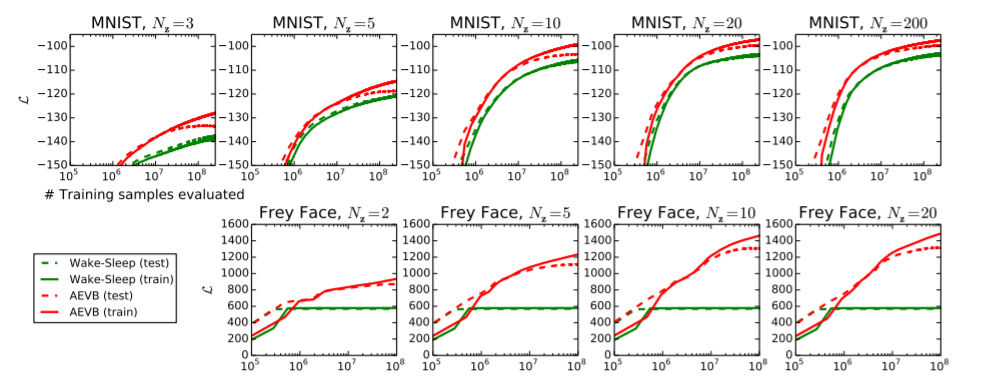
\includegraphics[clip, width=15cm]{../figures/comparison_WakeSleep}
    \caption{
        様々な潜在空間の次元\(N_z\)に対する,
        下限の最適化という観点での
        AEVBアルゴリズムとWake-Sleepアルゴリズムの比較。
        我々の手法は全ての設定で非常に早くかつより良い解に至っている。
        興味深いことに,
        潜在変数を増やしても過学習は起こらなかった。
        これは下限の正則化効果から説明される。
        縦軸は推定平均下限である。
        推定器のバリアンスは小さく(\(< 1\))無視できる。
        横軸は訓練データ数である。
        100万訓練データの計算には,
        40 GFLOPSで稼働するIntel Xeon CPUを用いて
        20--40分かかった。
        }
    \label{fig:comparison_WakeSleep}
\end{figure}


\paragraph{周辺尤度}

潜在空間が非常に低次元な場合は,
学習された生成モデルの周辺尤度を,
MCMC推定器を用いて推定することが可能になる。
周辺尤度の推定器に関しては,付録に詳しく示した。
符号器・復号器には隠れユニット数100,潜在変数3のニューラルネットワークを用いる。
高次元の潜在空間では信頼性が下がるためである。
また,データセットはMNISTを用いた。
詳細は付録に示すが,
AEVBとWake-Sleep法を
ハイブリッドモンテカルロサンプリング[DKPR87]を用いたモンテカルロEM法(MCEM法)と比較した。
訓練データのサイズとして,大きいものと小さいものに対し,
3つのアルゴリズムの収束速度を比較した。
図\ref{fig:comparison_MCMC}に結果を示した。

\begin{figure}
    \centering
    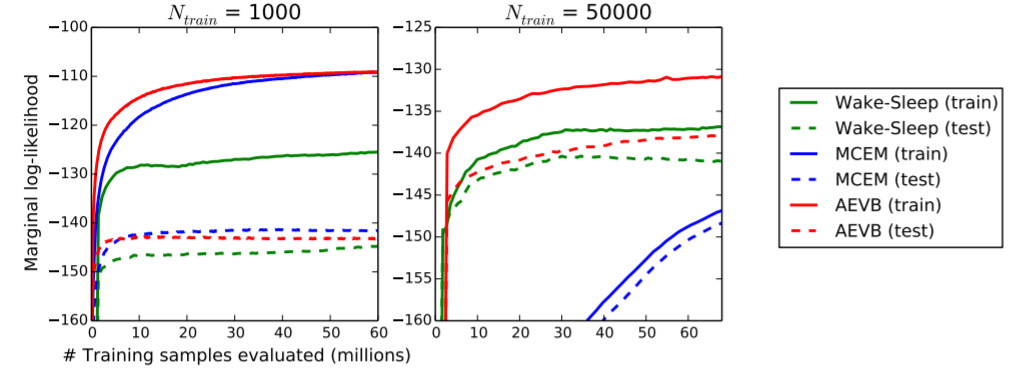
\includegraphics[clip, width=15cm]{../figures/comparison_MCMC}
    \caption{
        推定された周辺尤度についての,
        AEVBとWake-Sleepアルゴリズム,モンテカルロEM法との比較。
        モンテカルロEM法はオンライン学習のできるアルゴリズムではなく,
        (AEVBやWake-Sleep法とは異なり)
        MNISTデータセット全体に対して効率的に適用することができない。
        }
    \label{fig:comparison_MCMC}
\end{figure}


\paragraph{高次元データの可視化}

潜在空間を低次元(2次元など)とすれば,
学習させた符号器(認識モデル)を用いて高次元データを低次元の多様体に写像することができる。
付録AにMNISTとFrey Faceデータセットに対する2次元の潜在多様体を可視化したものを示した。



\section{結論}

本論文では,
連続型の潜在変数に対して効率的に近似推論を行うために,
変分下限についての新しい推定器,
確率的勾配変分ベイズ(SGVB)を導入した。
提案した推定器は標準的な確率的勾配法を用いて直接的に微分し最適化することができる。
また,各データに対し連続型の潜在変数があるようなi.i.dなデータセットに対して効率的に学習・推論を行うために,
近似推論モデルをSGVB推定器を用いて学習する,
自己符号化変分ベイズ(AEVB)アルゴリズムを導入した。
この理論の利点は実験結果に表れている。



\section{今後の展望}

SGVB推定器とAEVBアルゴリズムは,
連続型の潜在変数を考えるほとんど全ての学習・推論問題に適用することができるため,
今後の展望としては様々なものが挙げられる。

\begin{enumerate}[label=(\roman*)]
    \item
        深層ニューラルネットワーク(畳み込みネットワークなど)を符号器と復号器に用い,
        AEVBを用いて訓練を行うことによる,
        階層的な生成構造の学習
    \item
        時系列モデル(つまり動的ベイジアンネットワーク)
    \item
        大域的パラメータへのSGVBの適用
    \item
        複雑なノイズ分布の学習に対して有用となる,
        潜在変数のある教師あり学習
\end{enumerate}



\appendix

\section{可視化}

図\ref{fig:manifolds},\ref{fig:latent_spaces}にSGVBで学習を行ったモデルについて,
潜在空間と対応する観測空間の可視化を示した。

\begin{figure}[H]
    \centering
    \begin{minipage}{0.35\linewidth}
        \centering
        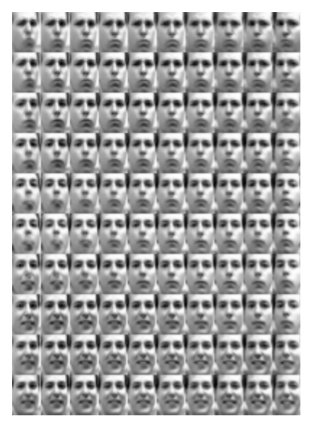
\includegraphics[clip, width=\linewidth]{../figures/FreyFace_manifold}
        \subcaption{学習されたFrey Faceの多様体}
        \label{fig:FreyFace_manifold}
    \end{minipage}
    \begin{minipage}{0.55\linewidth}
        \centering
        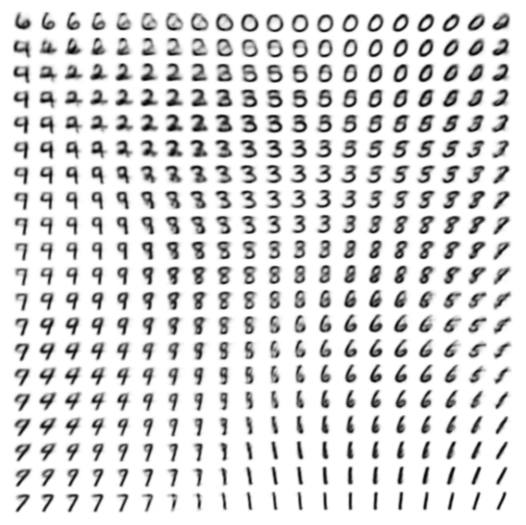
\includegraphics[clip, width=\linewidth]{../figures/MNIST_manifold}
        \subcaption{学習されたMNISTの多様体}
        \label{fig:MNIST_manifold}
    \end{minipage}
    \caption{
        AEVBで学習した2次元の潜在空間を持つ生成モデルの,
        学習されたデータの多様体の可視化。
        潜在空間の事前分布はガウス分布であるため,
        方眼状に線形に配置された座標を
        ガウス分布の逆累積分布関数によって変換することで
        潜在変数\(\bm{z}\)を得る。
        これらの\(\bm{z}\)の値それぞれに対し,
        学習した\(\theta\)について対応する\(p_{\theta} (\bm{x} | \bm{z})\)をプロットした。
        }
    \label{fig:manifolds}
\end{figure}

\begin{figure}[H]
    \centering
    \begin{minipage}{0.2\linewidth}
        \centering
        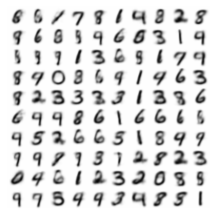
\includegraphics[clip, width=\linewidth]{../figures/latent_space_2D}
        \subcaption{2次元潜在空間}
        \label{fig:latent_space_2D}
    \end{minipage}
    \begin{minipage}{0.2\linewidth}
        \centering
        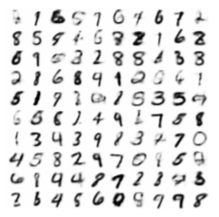
\includegraphics[clip, width=\linewidth]{../figures/latent_space_5D}
        \subcaption{5次元潜在空間}
        \label{fig:latent_space_5D}
    \end{minipage}
    \begin{minipage}{0.2\linewidth}
        \centering
        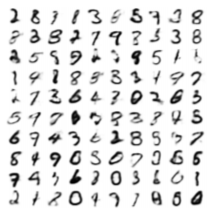
\includegraphics[clip, width=\linewidth]{../figures/latent_space_10D}
        \subcaption{10次元潜在空間}
        \label{fig:latent_space_10D}
    \end{minipage}
    \begin{minipage}{0.2\linewidth}
        \centering
        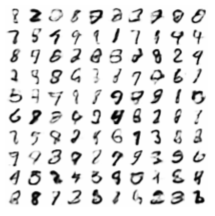
\includegraphics[clip, width=\linewidth]{../figures/latent_space_20D}
        \subcaption{20次元潜在空間}
        \label{fig:latent_space_20D}
    \end{minipage}
    \caption{
        様々な潜在空間の次元について,
        学習したMNISTの生成モデルからランダムにサンプリングしたもの。
        }
    \label{fig:latent_spaces}
\end{figure}



\section{ガウス分布に対する\(D_\mathrm{KL}(q_{\phi}({z}) || p_{\theta} ({z}))\)の解}

変分下限(最大化したい目的関数)はKL情報量の項を含んでいるが,
これは解析的に積分することで計算されることが多い。
ここでは,
事前分布\(p_{\theta} (\bm{z}) = \mathcal{N} (\bm{0},\ \bm{I})\)
かつ事後分布の近似\(q_{\phi} (\bm{z} | \bm{x}^{(i)})\)がガウス分布であるときの解を与える。
\(\bm{z}\)の次元を\(J\)とする。
\(\bm{\mu}\)と\(\bm{\sigma}\)をデータ\(i\)に対して計算された
変分平均と標準偏差とし,
\(\mu_j\)と\(\sigma_j\)でそれらのベクトルの\(j\)番目の要素を指すこととする。
このとき,
\begin{align*}
    \int q_{\theta} (\bm{z}) \log{p(\bm{z})} \dd{\bm{z}}
        & = \int \mathcal{N} (\bm{z}; \bm{\mu}, \bm{\sigma}^2) \log{\mathcal{N}(\bm{z}; \bm{0}, \bm{I})} \dd{\bm{z}} \\
        & = -\frac{J}{2} \log(2\pi) - \frac{1}{2} \sum_{j=1}^{J} (\mu_j^2 + \sigma_j^2)
\end{align*}
また,
\begin{align*}
    \int q_{\theta} (\bm{z}) \log{q_{\theta} (\bm{z})} \dd{\bm{z}}
        & = \int \mathcal{N} (\bm{z}; \bm{\mu}, \bm{\sigma}^2) \log{\mathcal{N}(\bm{z}; \bm{\mu}, \bm{\sigma}^2)} \dd{\bm{z}} \\
        & = -\frac{J}{2} \log(2\pi) - \frac{1}{2} \sum_{j=1}^{J} (1 + \log{\sigma_j^2})
\end{align*}
よって,
\begin{align*}
    -D_\mathrm{KL}(q_{\phi}(\bm{z}) || p_{\theta} (\bm{z}))
        & = \int q_{\theta} (\bm{z}) \qty(\log{p_{\theta} (\bm{z}) - \log{q_{\theta} (\bm{z})}}) \dd{\bm{z}} \\
        & = \frac{1}{2} \sum_{j=1}^{J} \qty{1 + \log((\sigma_j)^2) - (\mu_j)^2 - (\sigma_j)^2}
\end{align*}
本文で例示した通り,
認識モデル\(q_{\phi} (\bm{z} | \bm{x})\)を用いるときは,
\(\bm{\mu}\)と標準偏差\(\bm{\sigma}\)は\(\bm{x}\)と変分パラメータ\(\phi\)のみの関数となる。



\section{確率的符号器・復号器としてのMLP}

変分自己符号化器においては,
ニューラルネットワークが確率的符号器・復号器として用いられる。
符号器・復号器には,データとモデルの種類に応じて様々なものを用いることができる。
我々は比較的単純なニューラルネットワーク,所謂多層パーセプトロン(MLP)を用いた。
符号器にはガウス分布のパラメータを出力するMLPを,
復号器にはデータの種類に応じてガウス分布もしくはベルヌーイ分布のパラメータを出力するMLPを用いた。

\subsection{復号器にベルヌーイ分布のパラメータを出力するMLPを用いるとき}

このとき,\(p_{\theta} (\bm{x} | \bm{z})\)を,
\(\bm{z}\)から単層の隠れ層を持つ全結合ニューラルネットワークを用いて計算される多変量ベルヌーイ分布とする。
\begin{equation}
    \begin{split}
        & \log{p(\bm{x} | \bm{z})} = \sum_{i=1}^{D} x_i \log{y_i} + (1 - x_i) \cdot \log(1 - y_i) \\
        & \text{where} \quad
            \bm{y} = f_{\sigma} \qty(\bm{W}_2 \tanh(\bm{W}_1 \bm{z} + \bm{b}_1) + \bm{b}_2)
    \end{split}
\end{equation}
ここで,\(f_{\sigma} (.)\)は要素ごとのシグモイド活性化関数であり,
また,\(\theta = \qty{\bm{W}_1,\ \bm{W}_2,\ \bm{b}_1,\ \bm{b}_2}\)はMLPの重みとバイアスである。


\subsection{符号器・復号器にガウス分布のパラメータを出力するMLPを用いるとき}

このとき,符号器または復号器を共分散行列が対角成分のみを持つ多変量ガウス分布として,
\begin{equation}
    \begin{split}
        & \log{p(\bm{x} | \bm{z})} = \log{\mathcal{N}(\bm{x}; \bm{\mu}, \bm{\sigma}^2 \bm{I})} \\
        & \text{where} \quad \bm{\mu} = \bm{W}_4 \bm{h} + \bm{b}_4 \\
        & \log{\bm{\sigma}^2} = \bm{W}_5  \bm{h} + \bm{b}_5 \\
        & \bm{h} = \tanh(\bm{W}_3 \bm{z} + \bm{b}_3)
    \end{split}
\end{equation}
ここで,\(\qty{\bm{W}_3,\ \bm{W}_4,\ \bm{W}_5,\ \bm{b}_3,\ \bm{b}_4,\ \bm{b}_5}\)はMLPの重みとバイアスであり,
復号器として用いるときは\(\theta\)の一部となる。
このネットワークが復号器\(q_{\phi} (\bm{z} | \bm{x})\)として用いられるときは,
\(\bm{z}\)と\(\bm{x}\)が交換され,
重みとバイアスは変分パラメータ\(\phi\)となることに注意されたい。



\section{周辺尤度の推定器}

我々は,低次元空間(5次元以下)でかつ十分なサンプル数があるときにいい推定を与える周辺尤度の推定器を導出した。
\(p_{\theta} (\bm{x},\ \bm{z}) = p_{\theta} (\bm{z}) p_{\theta} (\bm{x} | \bm{z})\)
を生成モデルとし,
ここからサンプリングすることを考える。
データ\(\bm{x}^{(i)}\)に対して,
周辺尤度\(p_{\theta} (\bm{x}^{(i)})\)を推定する。

推定の過程は以下の3段階に分けられる。

\begin{enumerate}
    \item
        事後分布から,
        \(\grad_{\bm{z}} \log{p_{\theta} (\bm{z} | \bm{x})} = \grad_{\bm{z}} \log{p_{\theta} (\bm{z})} + \grad_{\bm{z}} \log{p_{\theta} (\bm{x} | \bm{z})}\)を用い,
        ハイブリッドモンテカルロ法などの
        勾配に基づくMCMC法によって,
        \(L\)個の値\(\qty{\bm{z}^{(l)}}\)をサンプリングする
    \item
        密度推定器\(q(\bm{z})\)にこれらのサンプル\(\qty{\bm{z}^{(l)}}\)を代入する
    \item
        再び事後分布から\(L\)個のサンプリングを行う。
        これらのサンプルを,\(q(\bm{z})\)と同様に,
        次の推定器に代入する。
        \begin{equation*}
            p_{\theta} (\bm{x}^{(i)}) \simeq \qty(\frac{1}{L} \sum_{l=1}^{L} \frac{q(\bm{z}^{(l)})}{p_{\theta} (\bm{z}) p_{\theta} (\bm{x}^{(i)} | \bm{z}^{(l)})})^{-1}
            \quad \text{where} \quad
            \bm{z}^{(l)} \sim p_{\theta} (\bm{z} | \bm{x}^{(i)})
        \end{equation*}
\end{enumerate}
この推定器の導出は以下の通りである。
\begin{align*}
    \frac{1}{p_{\theta} (\bm{x}^{(i)})}
        & = \frac{\int q(\bm{z}) \dd{\bm{z}}}{p_{\theta} (\bm{x}^{(i)})} \\
        & = \frac{\int q(\bm{z}) \frac{p_{\theta} (\bm{x}^{(i)},\ \bm{z})}{p_{\theta} (\bm{x}^{(i)},\ \bm{z})} \dd{\bm{z}}}{p_{\theta} (\bm{x}^{(i)})} \\
        & = \int \frac{p_{\theta} (\bm{x}^{(i)},\ \bm{z})}{p_{\theta} (\bm{x}^{(i)})} \frac{q(\bm{z})}{p_{\theta} (\bm{x}^{(i)},\ \bm{z})} \dd{\bm{z}} \\
        & = \int p_{\theta} (\bm{z} | \bm{x}^{(i)}) \frac{q(\bm{z})}{p_{\theta} (\bm{x}^{(i)},\ \bm{z})} \dd{\bm{z}} \\
        & \simeq \frac{1}{L} \sum_{l=1}^{L} \frac{q(\bm{z}^{(l)})}{p_{\theta} (\bm{z}) p_{\theta} (\bm{x}^{(i)} | \bm{z})} \\
        & \text{where} \quad \bm{z}^{(l)} \sim p_{\theta} (\bm{z} | \bm{x}^{(i)})
\end{align*}



\section{モンテカルロEM法}

モンテカルロEM法では符号器を用いず,
代わりに潜在変数の事後分布から,
その勾配を
\(\grad_{\bm{z}} \log{p_{\theta} (\bm{z} | \bm{x})} = \grad_{\bm{z}} \log{p_{\theta} (\bm{z})} + \grad_{\bm{z}} \log{p_{\theta} (\bm{x} | \bm{z})}\)
を用いて計算し,
サンプリングを行う。
モンテカルロEM法は10HMCリープフロッグステップから成り,
その学習率は,その引受率を90{\%}とし,得られたサンプルを用いて5ステップで重みを更新することで,自動的に調整される。
全てのアルゴリズムに対し,
パラメータはAdagradの学習率を用いて更新された
(焼きなまし法も用いた)。

周辺尤度は訓練データ及びテストデータの初めの1,000データから推定した。
ハイブリッドモンテカルロ法をリープフロッグステップを4とし,
各データに対し潜在変数の事後分布から50個をサンプリングした。



\section{完全変分ベイズ}

論文に記載の通り,
変分推論を,
潜在変数のみでなく
パラメータ\(\theta\)と潜在変数\(\bm{z}\)の両方を用いて行うことは可能である。
ここではその場合における推定器を導出しよう。

\(p_{\alpha} (\theta)\)を上記のパラメータに対する
ハイパーパラメータの事前分布とし,
\(\alpha\)をそのパラメータとする。
周辺尤度は次のように表される。
\begin{equation}
    \log{p_{\alpha} (\bm{X})}
        = D_\mathrm{KL} (q_{\phi} (\theta) || p_{\alpha} (\theta | \bm{X}))
            + \mathcal{L}(\phi; \bm{X})
\end{equation}
ここで,右辺第一項は真の事後分布から測ったその近似のKL情報量を表し,
\(\mathcal{L}(\phi; \bm{X})\)は周辺尤度の変分下限を表す。
\begin{equation}
    \mathcal{L}(\phi; \bm{X}) = \int q_{\phi} (\theta) \qty(\log{p_{\theta} (\bm{X})} + \log{p_{\alpha} (\theta)} - \log{q_{\phi} (\theta)}) \dd{\theta}
    \label{eq:variational_lower_bound_full_VB}
\end{equation}
KL情報量は非負のため,
これが下限となることに注意されたい。
近似分布が真の分布と完全に一致したとき,下限は真の周辺分布と一致する。
\(\log{p_{\theta} (\bm{X})}\)の項は各データの周辺尤度の和であり,
\(\log{p_{\theta} (\bm{X})} = \sum_{i=1}^{N} \log{p_{\theta} (\bm{x}^{(i)})}\)となって,
またこれの各項は次のように表される。
\begin{equation}
    \log{p_{\theta} (\bm{x}^{(i)})} = D_\mathrm{KL} (q_{\phi} (\bm{z} | \bm{x}^{(i)}) || p_{\theta} (\bm{z} | \bm{x}^{(i)})) + \mathcal{L}(\theta, \phi; \bm{x}^{(i)})
\end{equation}
ここで再び右辺第一項は真の事後分布から測ったその近似のKL情報量となっており,
\(\mathcal{L}(\phi; \bm{X})\)はデータ\(i\)の周辺尤度の変分下限を表す。
\begin{equation}
    \mathcal{L}(\theta, \phi; \bm{x}^{(i)}) = \int q_{\phi} (\bm{z} | \bm{x}) \qty(\log{p_{\theta} (\bm{x}^{(i)} | \bm{z})} + \log{p_{\theta} (\bm{z})} - \log{q_{\phi} (\bm{z} | \bm{x})}) \dd{\bm{z}}
    \label{eq:variational_lower_bound_full_VB_per_data}
\end{equation}
式(\ref{eq:variational_lower_bound_full_VB})と(\ref{eq:variational_lower_bound_full_VB_per_data})の
右辺の期待値は当然3つの別々の期待値の和として表すことができる。
また,\(p_{\theta} (\bm{x})\)と\(q_{\phi} (\bm{z} | \bm{x})\)がともにガウス分布であるなど,
この第二項と第三項は解析的に解くことができる場合もある。
一般化のため,ここではこれらの期待値は計算不可能であるとする。

ある緩い条件の下で(本文参照),
事後分布の近似\(q_{\phi} (\theta)\)と\(q_{\phi} (\bm{z} | \bm{x})\)に対し,
次のような条件付きサンプリング
\(\tilde{\bm{z}} \sim q_{\phi} (\bm{z} | \bm{x})\)
を次式のように再パラメータ化することができる。
\begin{equation}
    \tilde{\bm{z}} = g_{\phi} (\bm{\epsilon},\ \bm{x})
    \quad \text{with} \quad
    \bm{\epsilon} \sim p(\bm{\epsilon})
\end{equation}
ここで,\(p(\bm{\epsilon})\)と関数\(g_{\phi} (\bm{\epsilon},\ \bm{x})\)は次式を満たすように選ばれる。
\begin{align}
    \mathcal{L}(\theta, \phi; \bm{x}^{(i)})
        & = \int q_{\phi} (\bm{z} | \bm{x}) \qty(\log{p_{\theta} (\bm{x}^{(i)} | \bm{z})} + \log{p_{\theta} (\bm{z})} - \log{q_{\phi} (\bm{z} | \bm{x})}) \dd{\bm{z}}
        \notag \\
        & = \int p(\bm{\epsilon}) \eval{\qty(\log{p_{\theta} (\bm{x}^{(i)} | \bm{z})} + \log{p_{\theta} (\bm{z})} - \log{q_{\phi} (\bm{z} | \bm{x})})}_{\bm{z} = g_{\phi} (\bm{\epsilon},\ \bm{x}^{(i)})} \dd{\bm{\epsilon}}
    \label{eq:variational_lower_bound_epsilon}
\end{align}
同様のことが事後分布の近似\(q_{\phi} (\theta)\)に対しても行える。
\begin{equation}
    \tilde{\theta} = h_{\phi} (\bm{\zeta})
    \quad \text{with} \quad
    \bm{\zeta} \sim p(\bm{\zeta})
\end{equation}
ここで,上と同様に,
事前分布\(p(\bm{\zeta})\)と関数\(h_{\phi} (\bm{\zeta})\)を,
次式が成立するように選ぶ。
\begin{align}
    \mathcal{L}(\phi; \bm{X})
        & = \int q_{\phi} (\theta) \qty(\log{p_{\theta} (\bm{X})} + \log{p_{\alpha} (\theta)} - \log{q_{\phi} (\theta)}) \dd{\theta}
        \notag \\
        & = \int p(\bm{\zeta}) \eval{\qty(\log{p_{\theta} (\bm{X})} + \log{p_{\alpha} (\theta)} - \log{q_{\phi} (\theta)})}_{\theta = h_{\phi} (\bm{\zeta})} \dd{\bm{\zeta}}
    \label{eq:variational_lower_bound_zeta}
\end{align}
簡単のため,\(f_{\phi} (\bm{x},\ \bm{z},\ \theta)\)を用いて次のように略記する。
\begin{equation}
    f_{\phi} (\bm{x},\ \bm{z},\ \theta) = N \cdot \qty(\log{p_{\theta} (\bm{x} | \bm{z})} + \log{p_{\theta} (\bm{z})} - \log{q_{\phi} (\bm{z} | \bm{x})}) + \log{p_{\alpha} (\theta)} - \log{q_{\phi} (\theta)}
    \label{eq:shorthand}
\end{equation}
式(\ref{eq:variational_lower_bound_zeta})と(\ref{eq:variational_lower_bound_epsilon})
を用いて,
データ\(\bm{x}^{(i)}\)に対する変分下限のモンテカルロ推定を行うと,
\begin{equation}
    \mathcal{L}(\phi; \bm{X}) \simeq \frac{1}{L} \sum_{l=1}^{L} f_{\phi} \qty(\bm{x}^{(l)},\ g_{\phi} (\bm{\epsilon}^{(l)},\ \bm{x}^{(l)}),\ h_{\phi} (\bm{\zeta}^{(l)}))
    \label{eq:variational_lower_bound_per_data_MC}
\end{equation}
ここで,\(\bm{\epsilon} \sim p(\bm{\epsilon}),\ \bm{\zeta}^{(l)} \sim p(\bm{\zeta})\)である。
推定器は\(p(\bm{\epsilon})\)と\(p(\bm{\zeta})\)からのサンプリングにしか依存せず,
それらは\(\phi\)に依存しないため,
この推定器は\(\phi\)について微分可能である。
得られる確率的勾配はSGDやAdagrad[DHS10]などの確率的最適化手法とともに用いられ
る。
確率的勾配を計算する基本的なアプローチについては,
アルゴリズム\ref{algo:AEVB_minibatch}を参照されたい。


\subsection{例}

パラメータと潜在変数の事前分布を標準ガウス分布
\(p_{\alpha} = \mathcal{N}(\bm{z}; \bm{0}, \bm{I}),\ p_{\theta} (\bm{z}) = \mathcal{N}(\bm{z}; \bm{0}, \bm{I})\)
とする。
このとき,事前分布にパラメータはないことに注意されたい。
また,真の事後分布も近似的に共分散行列が対角成分しか持たないガウス分布となると仮定する。
このとき,
変分近似事後分布は共分散行列が対角成分しか持たない多変量ガウス分布とすることができ,
\begin{align}
    & \log{q_{\phi} (\theta)} = \log{\mathcal{N}(\theta; \bm{\mu}_{\theta}, \bm{\sigma}_{\theta}^2 \bm{I})} \notag \\
    & \log{q_{\phi} (\bm{z} | \bm{x})} = \log{\mathcal{N}(\bm{z}; \bm{\mu}_{\bm{z}}, \bm{\sigma}_{\bm{z}}^2 \bm{I})}
\end{align}
ここで,\(\bm{\mu}_{\bm{z}}\)と\(\bm{\sigma}_{\bm{z}}\)は依然\(\bm{x}\)の何らか関数である。
これらはガウス分布であるため,
変分近似事後分布をパラメータ化でき,
\begin{align*}
    & q_{\phi} (\theta)
        \quad \text{as} \quad
        \tilde{\theta} = \bm{\mu}_{\theta} + \bm{\sigma}_{\theta} \odot \bm{\zeta}
        \qquad \text{where} \quad
        \bm{\zeta} \sim \mathcal{N}(\bm{0},\ \bm{I}) \\
    & q_{\phi} (\bm{z} | \bm{x})
        \quad \text{as} \quad
        \tilde{\bm{z}} = \bm{\mu}_{\bm{z}} + \bm{\sigma}_{\bm{z}} \odot \bm{\epsilon}
        \qquad \text{where} \quad
        \bm{\epsilon} \sim \mathcal{N}(\bm{0},\ \bm{I})
\end{align*}
ここで,\(\odot\)は要素ごとの積を表す。
これらは上で定義した下限の式(式(\ref{eq:shorthand}),(\ref{eq:variational_lower_bound_per_data_MC}))に対して用いることができる。

このとき,
このモデルでは\(p_{\alpha} (\theta),\ p_{\theta} (\bm{z}),\ q_{\phi} (\theta),\ q_{\phi} (\bm{z} | \bm{x})\)がガウス分布であり,
\(f_{\phi}\)の4つの項が解析的に求まるので,
よりバリアンスの小さい別の推定器を構成することができる。
得られる推定器は次式のようになる。
\begin{align}
    \mathcal{L}(\phi; \bm{X})
        & \simeq \frac{1}{L} \sum_{l=1}^{L} N \cdot \qty(
            \frac{1}{2} \sum_{j=1}^{J} (1 + \log((\sigma_{\bm{z}, j}^{(l)})^2) - (\mu_{\bm{z}, j}^{(l)})^2 - (\sigma_{\bm{z}, j}^{(l)})^2)
            + \log{p_{\theta} (\bm{x}^{(i)} \bm{z}^{(i)})}
            )
        \notag \\
        & \ \qquad
            + \frac{1}{2} \sum_{j=1}^{J} \qty(1 + \log((\sigma_{\theta, j}^{(l)})^2) - (\mu_{\theta, j}^{(l)})^2 - (\sigma_{\theta, j}^{(l)})^2)
\end{align}
\(\mu_j^{(l)}\)と\(\sigma_j^{(l)}\)は単にベクトル\(\bm{\mu}^{(i)}\)と\(\bm{\sigma}^{(i)}\)の\(j\)番目の要素を表している。


\begin{algorithm}
    \caption{
        提案した推定器を用いて確率的勾配を計算する疑似コード。
        \(f_{\phi},\ g_{\phi},\ h_{\phi}\)の意味については本文参照のこと。
        }
    \label{algo:pseudo_SGD}
    \begin{algorithmic}
        \REQUIRE \(\phi\) (Current value of variational parameters)
        \STATE \(g \leftarrow 0\)
        \FOR{\(l\) is 1 to \(L\)}
            \STATE \(\bm{x} \leftarrow \text{Random draw from dataset } \bm{X}\)
            \STATE \(\bm{\epsilon} \leftarrow \text{Random draw from prior } p(\bm{\epsilon})\)
            \STATE \(\bm{\zeta} \leftarrow \text{Random draw from prior } p(\bm{\zeta})\)
            \STATE \(g \leftarrow g + \frac{1}{L} \grad_{\phi} f_{\phi} (\bm{x}, g_{\phi} (\bm{\epsilon}, \bm{x}), h_{\phi} (\bm{\zeta})) \)
        \ENDFOR
        \RETURN \(g\)
    \end{algorithmic}
\end{algorithm}



\end{document}
